\lecture{23}{2025-05-13}{linear codes}{}
\begin{parag}{Last Week}
    Last week, we did linear algebra but in modulo. We use finite field with linear algebra like this:
    \begin{align*} \vec{x} \in \mathbb{F}^n \end{align*}
    We also work with subspace:
    \begin{align*} S \subseteq \mathbb{F}^n \end{align*}
\end{parag}


\section{Vector Spaces and Linear Codes}

\begin{parag}{What and why Linear codes?}
    \begin{itemize}
        \item Linear code have more structure
    \end{itemize}
    We use that structure to simplify our tasks,  notably:
    \begin{itemize}
        \item To determine the code's performance ($d_{min}$ in particular)
        \item To simplify the encoding
        \item To simplify the decoding
    \end{itemize}
    
\end{parag}
\begin{parag}{Linear Code}
    \begin{definition}
        A block code is a \textbf{linear code} if the codewords form a subspace of $\mathbb{F}^n$ for some finite field $\mathbb{F}$.
    \end{definition}
    \begin{subparag}{Example}
        Let $\mathcal{C} \subset \mathbb{F}_2^7$ be the block code that consists of the listed codewords. Is it linear?
        
        \begin{center}
        \begin{tabular}{|c|}
            Code $\mathcal{C}$ \\
            $\vec{v}_1 = 0000000$ \\
            $\vec{v}_2 = 0011100$ \\
            $\vec{v}_3 = 0111011$ \\
            $\vec{v}_4 = 1110100$ \\
            $\vec{v}_5 = 1101000$ \\
            $\vec{v}_6 = 1001111$ \\
            $\vec{v}_7 = 1010011$ \\
        \end{tabular}
        \end{center}
        
        We have that:
        \begin{align*} 
            \vec{c}_4 &=  \vec{c}_1 + \vec{c}_2\\
            \vec{c}_5 &=  \vec{c}_1 + \vec{c}_3\\
            \vec{c}_6 &=  \vec{c}_2 + \vec{c}_3\\
            \vec{c}_7 &=  \vec{c}_1 + \vec{c}_2 + \vec{c}_3\\
        \end{align*}
        Therefore $\mathcal{C} =  \text{span}\left(\vec{c}_1, \vec{c}_2, \vec{c}_3\right) \subset \mathbb{F}_2^7$ is a linear code (over the finite field $\mathbb{F}_2$).
    \end{subparag}
    \begin{subparag}{How to check}
        To check if a code is a linear code, we juste have to check if it is a subspace, is there the zero vector is in.\\
        The number of codeword must be $2^k$ for some $k$. (you cannot be a subspace if you are not the cardinality to the power $k$). After having check those two, we don't know if it is a subspace, those are only a necessity.\\
        To check we need to find a basis.
    \end{subparag}
\end{parag}

\begin{parag}{Size vs Dimension}
    We have seen that a $k$-dimensional subspace of $\mathbb{F}^n$ has cardinality $\left[\text{card}\left(\mathbb{F}\right)\right]^k$. (Count the number of linear combinations you can form with the vectors that form the basis, with coefficients in $\mathbb{F}$)
    \begin{framedremark}
        If the size of a binary block code is not of the form $2^k$, then the code is not linear.
    \end{framedremark}
\end{parag}

\begin{parag}{Hamming weight (not distance)}
    \begin{definition}
    Let $\vec{x} =  \left(x_1, \ldots, x_n\right)$ be an $n$-tuple with components in a finite field.\\
    The \important{Hamming weight} of $\vec{x}$, denoted $w\left(\vec{x}\right)$, is the number of its non-zero components in $\left(x_1, \ldots, x_n\right)$ , i.e.
    \begin{align*} w\left(\vec{x}\right) = d\left(\left(0, \ldots, 0\right), \left(x_1, \ldots, x_n\right)\right) \end{align*}
    \end{definition}
    
\end{parag}
\begin{parag}{Exercise (Academic question)}
    In the definition of Hamming weight, we are requiring that the components of $\vec{x}$ take value in a (finite) field $\mathbb{F}$ . Why?
    \begin{subparag}{Solution}
       If there are not, there is no guarantee that the alphabet contains the $0$ element.\\
       Recall that in a finite field $\mathbb{F}$, no matter how we label its elements, one is the 0 element ( the identity element with respect to addition). Hence the hamming weight is well defined. 
    \end{subparag}
    \begin{subparag}{Example}
        \begin{itemize}
        \item The weight of $\left(1, 0, 1, 1, 0\right)$ is $3$ 
        \item The weight of $\left(3, 0, 4, 1, 1, 2\right)$ is $5$
        \end{itemize}
    \end{subparag}
\end{parag}
\begin{parag}{Theorem}
    \begin{theoreme}
    The minimum distance of a linear code $\mathcal{C}$ is the smallest weight of a codeword in $\mathcal{C}$, zero-vector excluded, i.e.:
    \begin{align*} d_{min}\left(\mathcal{C}\right) =  \text{min}_{\vec{c}\in \mathcal{C}: \vec{c}\neq \vec{0}} w\left(\vec{c}\right)\end{align*}
    \end{theoreme}
    \begin{subparag}{note before the proof}
        In the proof that follows, we use the following facts:
        \begin{itemize}
            \item For all $\vec{u} \vec{v} \in \mathbb{F}$ 
                \begin{align*} d\left(\vec{u}, \vec{v}\right) = w\left(\vec{u} - \vec{w}\right) \end{align*}
                Let us proof this:
                \begin{align*}  
                    d\left(\vec{u}, \vec{v}\right) = \sum_{i =  1}^{n} d\left(u_i, v_i\right)\\
                    w\left(\vec{u} - \vec{v}\right) =  \sum_{i =  1}^{n} w\left(u_i - v_i\right)
                \end{align*}
                Therefore:
                \begin{align*} 
                    d\left(u_i, v_i\right) =  w\left(u_i - v_i\right)
                \end{align*}
                ($\vec{u}$ and $\vec{v}$ are different at position $i$ if and only if $\vec{u}-\vec{v}$  is non-zero at position $i$)
            \item Let $f: \mathcal{B} \to \mathbb{R}$ be an arbitrary function and $A \subseteq B$ be finite sets. Then
                \begin{align*} \text{min}_{x \in \mathcal{A}}f\left(x\right) \geq \text{min}_{x \in \mathcal{B}}f\left(x\right) \end{align*}
                (We might find a smaller minimum if we enlarge the set)
        \end{itemize}
    \end{subparag}
    \begin{subparag}{Proof}
        \begin{align*} d_{min}\left(\mathcal{C}\right) &=  \text{min}_{\vec{u}, \vec{v} \in \mathcal{C}: \vec{u}\neq \vec{v}}d\left(\vec{u}, \vec{v}\right) \\
        &= \text{min}_{\vec{u}, \vec{v} \in \mathcal{C}: \vec{u}\neq \vec{v}} w\left(\vec{u}-\vec{v}\right)\\
        &\geq \text{min}_{\vec{c} \in \mathcal{C}: \vec{c} \neq \vec{0}} w\left(\vec{c}\right)\end{align*}
        Which leads to:
        \begin{align*} 
           w \text{min}_{\vec{c}\in \mathcal{C}: \vec{c} \neq \vec{0}} \left(\vec{c}\right)&=  \text{min}_{\vec{c}\in \mathcal{C}: \vec{c} \neq \vec{0}} d\left(\vec{c}, 0\right)\\
                                                                                           &\geq  \text{min}_{\vec{c}\in \mathcal{C}: \vec{c} \neq \vec{0}}  d\left(\vec{c}, \vec{v}\right) \\
                                                                                           &= d_{min}\left(\mathcal{C}\right)
        \end{align*}
    \end{subparag}
\end{parag}


\begin{parag}{Example}
    Let us take the code $\mathcal{C} \subseteq \mathbb{F}_2^n$:
    \begin{align*} \mathcal{C} =  \left\{\text{all sequences with an even number of 1's}\right\} \end{align*}
    In the yellow universe we have:
    \begin{align*} \left\{\vec{s}: s_1 + s_2 + \ldots s_n = 0\right\} \end{align*}
    Then the question is $\dim \left(\mathcal{C}\right) = n-1$, why? We get rid of the yellow universe which is like the ``noyau'' in French.\\
    Now we search for $d_{min}\left(\mathcal{C}\right) =  2$ which is the smallest number (except $0$) with have a even number of $1$ which is  2.
    \begin{framedremark}
        Here we see that this meets singleton bound, which means that this is a very good code.\\
        In this example, linearity allows us to determine $d_{min}$ via deductive reasoning rather than by inspection. 
    \end{framedremark}
\end{parag}
\begin{parag}{Exercise}
    if is the subset of $\mathbb{F}_2^n$ that consists of two codewords, namely $\left(0, \ldots, 0\right)$ and $\left(1, \ldots, 1\right)$.\\
    Determine $k$ and $d_{min}$.
    \begin{subparag}{Solution}
        The code is linear: it is the subspace of $\mathbb{F}_2^n$ spanned by $\left(1, \ldots, 1\right)$ (because the $\vec{0}$ is just $0 \cdot  \left(1, \ldots, 1\right)$.\\
        Therefore we can find that $k =  1$. (one vector)\\
        $d_{min} =  n$ (the weight of the only non zero vector) (which is always not equal to $1$)
    \end{subparag}
\end{parag}
    The above two codes are not terribly useful, but they have an interesting property shared by the next code which is even less useful:
\begin{parag}{Exercise again}
    $\mathbb{F}_2^n$ satisfies the definition of a linear code\\
    Determine $k$ and $d_{min}$.
    \begin{subparag}{Solution}
        $k =  n$ we can juste take the ``vecteur unitaire'' and the each one of those vector cannot be written using other vector.\\
        $d_{min} = 1$ which is vectors with only one $1$.
    \end{subparag}
\end{parag}
The above three code families fulfill the singleton bound with equality. Hence, they are MDS codes, Moreover, they are also linear codes.\\
No other family of binary linear codes is MDS\\
No other family of binary linear codes is $MDS$.\\
But there are non binary codes that are MDR, e.g. The family of Reed solomon codes (studied next week)

\subsubsection{Generator Matrix}

\begin{parag}{Definition}
    \begin{definition}
        Let $\left(\vec{c}_1, \ldots, \vec{c}_k\right)$ be a basis of a linear code $\mathcal{C} \subset \mathbb{F}^n$ over some finite field $\mathbb{F}$. The $k \times m $ matrix that has $\vec{c}_i$  as its $i$\Th row is called  \important{generator matrix} of $\mathcal{C}$.
    \end{definition}
    \begin{subparag}{Example}
        $\left(\vec{c}_1, \vec{c}_2, \vec{c}_3\right)$ form a basis for $\mathcal{C}$. Therefore:
        \begin{align*} 
            G =  \begin{pmatrix} \vec{c}_1 \\ \vec{c}_2 \\ \vec{c}_3 \end{pmatrix} = \begin{pmatrix} 0 & 0 & 1 & 1 & 1 & 0 & 0 \\ 0  & 1 & 1 & 1 & 0 & 1 & 1 \\ 1 & 1 & 1 & 0 & 1 & 0 & 0 \end{pmatrix} 
        \end{align*}
        Is a generator matrix of $\mathcal{C}$.
    \end{subparag}
\end{parag}
\begin{parag}{Encoding}
    A $k \times n$ generator matrix specifies an \important{encoding map} that sends an \important{information vector} $\vec{u} \in \mathbb{F}^k$ to the corresponding $\vec{c}= \vec{u}G$.
    \begin{center}
        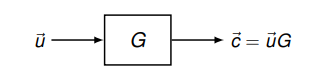
\includegraphics[scale=1.1]{12025-05-13.png}
    \end{center}
    So the way to encode is really to multiply the $\vec{u}$ by the matrix $G$ and \important{this is} the codeword
    \begin{subparag}{Example}
        \begin{align*} 
            \vec{u} =  \left(1, 0, 1\right) \to \vec{c} =  \left(1, 0, 1\right) \begin{pmatrix} 0 & 0 & 1 & 1 & 1 & 0 & 0 \\ 0 & 1 & 1 & 1 & 0 & 1 & 1 \\ 1 & 1 & 1 & 0 & 1 & 0 & 0 \end{pmatrix} \\
            = \left(1, 1, 0, 1, 0, 0, 0\right)
        \end{align*}
    \end{subparag}
    
    \begin{framedremark}
        A generator matrix is \textbf{not unique}  you can take for a matrix:
        \begin{align*} G_1 =  \begin{pmatrix} \vec{c}_1 \\ \vec{c}_2 \\ \vec{c}_3 \end{pmatrix}  \end{align*}
        Or:
        \begin{align*} \begin{pmatrix} \vec{c}_1 \\ \vec{c}_1 + \vec{c}_2 \\ \vec{c}_1 + \vec{c}_3 \end{pmatrix}  \end{align*}

    \end{framedremark}
\end{parag}
\begin{parag}{Exercise}
    How many generator matrices for a binary linear code of block length $n = 7$ and dimension $k =  3$.
    \begin{subparag}{Solution}
        It is the number of lists that form a basis. A q-ary linear code of dimension $k$ has $q^k$ codewords and the number of bases is:
        \begin{align*} \left(q^k - 1\right)\left(q^k-q\right)\ldots\left(q^k-q^{k-1}\right) \end{align*}
        For a binary code  ($q= 2$) we have:
        \begin{align*} \left(2^3 - 1\right)\left(2^3 - 2\right)\left(2^3 - 2\right) = 7 \cdot  6 ç 4 = 168 \end{align*}
    \end{subparag}
\end{parag}
\begin{parag}{Transmitter (big picture)}
    Here we got rid of the crypto part and we assumed we already have nice bits to transfer.
    \begin{center}
        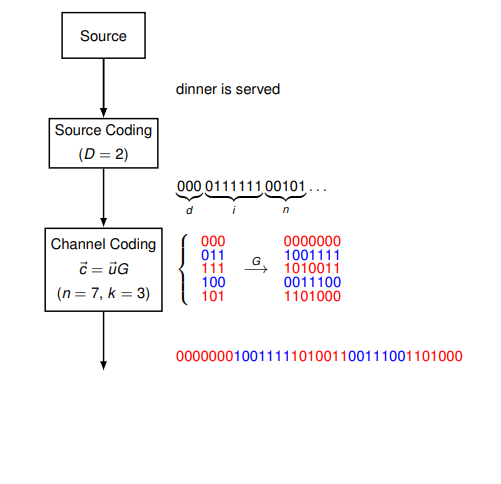
\includegraphics[scale=0.6]{22025-05-13.png}
    \end{center}
    \begin{framedremark}
        The crypto module would by between the source coding and the channel coding
    \end{framedremark}
\end{parag}


\begin{parag}{Exercice}
    given the code $\mathcal{C}$ (the same as before), is $\left(\vec{c}_2 + \vec{c}_3, \vec{c}_1 + \vec{c}_2, \vec{c}_1\right)$ a basis of $\mathcal{C}$?\\
    if yes,\\
    \begin{itemize}
        \item Specify the generator matrix
        \item Explicitly specify the map $u_1u_2u_3 \to c_1c_2c_3c_4c_5c_6c_7$
    \end{itemize}
    

\end{parag}

\begin{parag}{Systematic form}
    the above matrix $G'$ is in systematic form
    \begin{definition}
    A generator matrix $G_s$ is in \important{systematic form} if:
    \begin{align*} G_s =  \left(I_k, P_{k \times\left(n-k\right)}\right) \end{align*}
    \end{definition}
    Notice that a systematic generator matrix is a matrix in reduced echelon form.\\
    When the generator matrix is in systematic form, each codeword is written as 
    \begin{align*} \vec{c} =  \vec{u}G_s =  \left(u_1, \ldots, u_k, c_{k+1}, \ldots, c_n\right) \end{align*}
\end{parag}
\begin{parag}{How to find the systematic form}
    \begin{enumerate}
        \item Find a basis $\{\vec{c}_1, \ldots , \vec{c}_k\}$ of $\mathcal{C}$
        \item Form the generator matrix: $G =  \begin{pmatrix} \vec{c}_1 \\ \vdots \\ \vec{c}_k \end{pmatrix} $
        \item Row-reduce $G$ (Gaussian elimination on rows) to obtain a matrix in reduced echelon form.
    \end{enumerate}
    
    
\end{parag}

